\chapter{\nmu Modélisation long terme de signaux sonores} \label{chap:modeles}

La plupart des modèles de sons utilisés dans la littérature sont des modèles à court terme. Les raisons de ce choix de conception sont nombreuses et seront détaillées ci-après. Une originalité de mon travail de recherche a été d'étudier les limitations de ce type d'approche et de contribuer à des alternatives qui, sans être totalement satisfaisantes à ce jour, nous permettent de mieux comprendre les défis scientifiques et techniques pour parvenir à une modélisation des signaux sonores qui soit à la fois fidèle et expressive.

\section{ \nmu Préambule}

On considérera ici qu'un signal sonore est un signal à valeurs réelles à temps discret, échantillonné à une fréquence de 40 kHz environ. Ce signal peut provenir d'une version quantifiée, mais on supposera que le pas de quantification est suffisamment réduit pour n'introduire qu'une dégradation perceptivement négligeable. On notera ce signal $s[n]$, il peut être observé sur un intervalle de temps donné, correspondant à un certain nombre d'échantillons temporels $s[n], 0<n<N-1$ souvent appelé intervalle d'observation, support ou encore champ réceptif. Je n'utiliserai pas ce document dans la version continue du signal, l'expression $f(x)$ devant donc se comprendre comme l'application d'une fonction $f$ à un signal $x$.

\begin{marginfigure}
  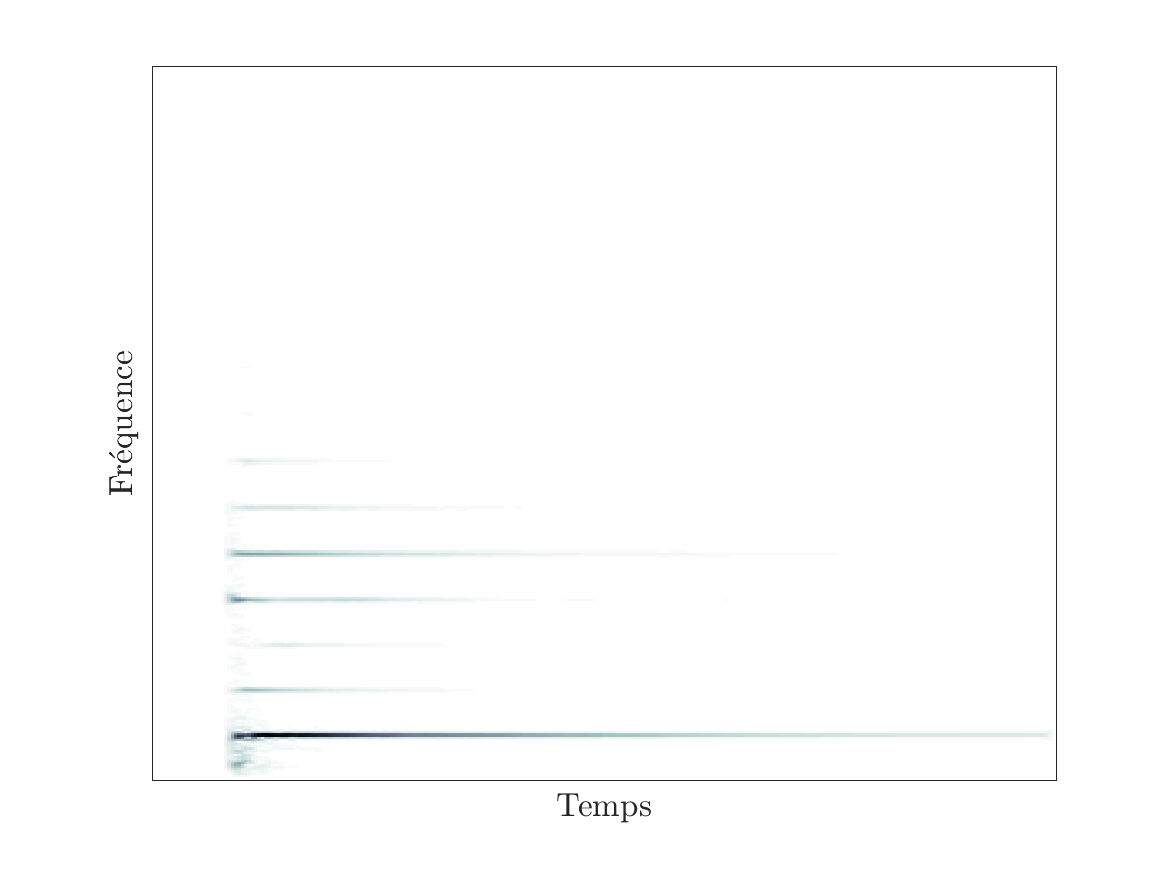
\includegraphics[width=\textwidth]{pianoSpec}
  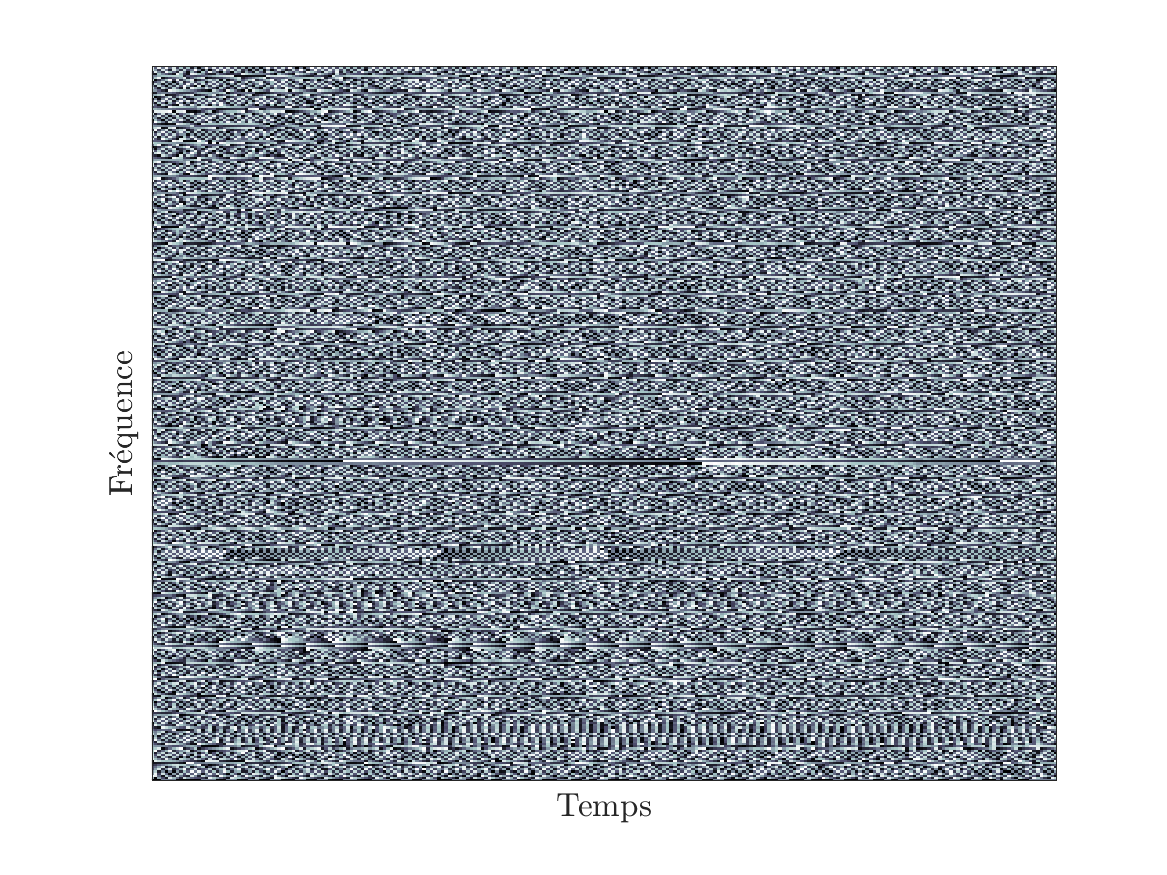
\includegraphics[width=\textwidth]{pianoPhase}
  \caption{Signal temporel ou forme d'onde d'une note de piano.}
  \label{fig:onde}
\end{marginfigure}

Également, le terme modélisation étant fortement polysémique, précisons l'usage qui sera fait du terme \og modèle de son \fg. Un modèle de son est une représentation du signal sonore qui permet de modifier ce signal d'une manière qui soit d'intérêt pour une tâche donnée et ce de manière cohérente avec certaines contraintes motivées par 1) des considérations physiques ou 2) la perception qu'en aurait un être humain. On notera $Pe(x)$, l'opérateur de perception humaine du signal $x$.  Le modèle est utilisé en considérant deux étapes de transformation, respectivement appelées \og analyse \fg et \og synthèse \fg. La phase d'analyse $A$, à partir d'un signal $x$, produit un modèle $X$ et la phase de synthèse $S$ permet, à partir de ce modèle $X$, de produire un signal $\tilde{x}=Sy(An(x))$.

Trois critères d'évaluation émergent alors pour qualifier ce modèle :
\begin{enumerate}
  \item \textbf{fidélité} : un modèle fidèle est capable de ne pas produire d'artefacts. Ce critère peut s'exprimer formellement de la manière suivante : $Pe(x) \sim Pe(\tilde{x})$.
  \item \textbf{expressivité} : un modèle expressif est capable de mettre à disposition des mécanismes de manipulation tels que la modification du modèle produise une modification cohérente de la perception du signal résultant. Ce critère peut s'exprimer formellement de la manière suivante : $Pe(Sy(X')) \sim Pe'(Sy(X))$.
  \item \textbf{versatilité} : un modèle versatile s'applique à tout type de signal sonore d'intérêt, \textit{i.e.} les conditions de fidélité et d'expressivité sont remplies pour tout signal $x$ d'intérêt pour une tâche donnée.
\end{enumerate}
\marginnote{
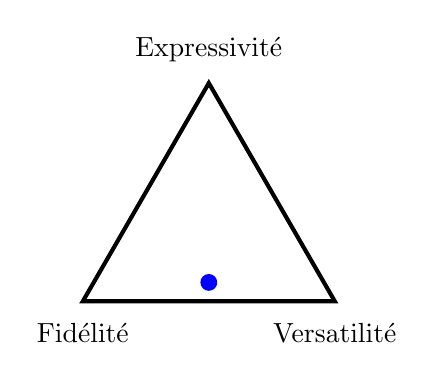
\begin{tikzpicture}[scale=0.8, label distance=1.5mm]
    \coordinate[label=below:Fidélité]  (A) at (0,0);
    \coordinate[label=below:Versatilité] (B) at (4,0);
    \coordinate[label=above:Expressivité] (C) at (2,3.464);
    \draw [line width=1.5pt] (A) -- (B) -- (C) -- cycle;
  \draw [blue, fill=blue, line width=1.5pt] (2,.3) circle [radius=.1 cm];
  \end{tikzpicture}
  La forme d'onde est modèle de son versatile et fidèle mais d'une expressivité limitée.
}
Avec ces trois critères d'évaluation, se dessine ici un triangle de contraintes qui nous permettra d'apprécier le compromis inhérent au choix  de chacun des modèles que nous discuterons. Par exemple, la forme d'onde est un modèle versatile et fidèle mais d'une expressivité limitée.

L'intuition ici, largement suivie dans la communauté des sciences des données est que, pour tout processus observable, il existe un modèle de ce processus pour lequel des manipulations basé sur des opérateurs mathématiques simples dans le domaine transformé \og font sens \fg dans le domaine \fg signal \og d'origine. On jugera alors la qualité du modèle par sa capacité à proposer de nouvelles réalisations du processus modélisé qui soient plausibles, c'est-à-dire perceptivement valides. Par exemple, en considérant le signal temporel, on peut aisément manipuler l'intensité perçue en multipliant tout les échantillons par une constante. Ce modèle ne permet par contre pas dans le cas général de manipuler aisément la hauteur perçue.

Cette approche se distingue clairement des approches dites \og modèles physiques \fg qui modélisent explicitement le processus mécanique, la qualité du son étant alors censée être la résultante d'une bonne modélisation du système physique dont la mise en vibration est à l'origine du signal sonore d'intérêt. Le distinguo est ici fait sur l'objet d'intérêt, à savoir que l'on s'intéresse aux propriétés du signal et non celles de la source. Ceci ne veut pas dire que l'on ne puisse pas, avec une approche sciences des données, se focaliser sur le signal d'un type de source sonore en particulier. Mais, dans ce cas, on s'attachera à exploiter les régularités du signal pour motiver notre modèle.

Dans la communauté traitement du signal, on parle souvent de modèle paramétrique, dans le sens où le modèle dispose d'un ensemble réduit de paramètres qui peuvent être explicitement manipulés pour influer sur le son modélisé. L'usage du terme \og paramétrique \fg est néanmoins à mon avis peu clair, et utilisé avec plus ou moins de bonheur dans la littérature. Je préférerai donc à ce terme le distinguo entre \og modèle \fg et \og transformée \fg. Un modèle expose donc pour moi un ensemble de paramètres manipulables, une transformée étant plutôt un outil de description. Ceci n'empêche pas qu'une transformée puisse avoir un modèle sous-jacent, ni que les étapes d'analyse et/ou de synthèse d'un modèle ne se basent sur une ou des transformées.

Précisons maintenant l'intervalle temporel dénommé par \og long terme \fg. Cela désignera ici une durée à partir de laquelle le signal sonore ne peut plus raisonnablement être considérée comme stationnaire.

De par nos connaissances sur les propriétés physiques de l'organe phonatoire, il est par exemple commun de considérer que le signal de parole est localement stationnaire sur un intervalle de 25 ms. Comme on peut le voir sur la Figure \ref{fig:speech} montrant des spectrogrammes de vocalisations humaines\cite{ladefoged2014course}, dès que l'on considère des consonnes, ou lorsque la prosodie évolue de manière conséquente, le signal sonore produit par l'organe vocal n'est plus stationnaire. Il me paraît donc plus juste de motiver ce choix par l'assertion suivante : \og il est raisonnable d'approximer le signal de parole avec un modèle stationnaire par morceaux à partir du moment où ces morceaux sont d'une durée inférieure à 25ms \fg.

\begin{marginfigure}
  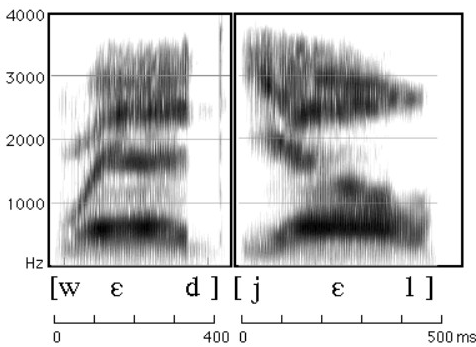
\includegraphics[width=\textwidth]{phonemesCrop}
  \caption{Spectrogrammes de vocalisations humaines.}
  \label{fig:speech} % Issue de l'ouvrage "A Course In Phonetics" de Ladefoged publié en 2006,  http://www.cog.jhu.edu/courses/325-f2004/ladefoged/course/chapter8/figure8.html
\end{marginfigure}

La dénomination \og long terme \fg  étant dépendante du degré de stationarité du signal étudié, il n'est donc pas possible de fixer une durée pour tout type de signaux sonores à partir de laquelle la dénomination \og long terme \fg est appropriée. On considérera néanmoins dans les études discutées dans ce document qu'un intervalle de temps  \og long terme \fg désigne un intervalle de temps supérieur ou égal à la seconde.

\section{ \nmu Typologie sonore} \label{sec:typologie}

Il est bien entendu que même si l'on souhaite que notre modèle soit versatile, on ne souhaite pas nécessairement que notre modèle soit capable de modéliser tout les signaux possibles. On supposera donc que certaines propriétés d'invariance existent, c'est-à-dire que même si une seconde de son échantillonnée à 44kHz est représentée dans $R^{44000}$, les paramètres du modèles\footnote{Ou variables latentes, ou encore code...} évoluent dans un espace de dimension beaucoup plus réduit. Je considère ce postulat raisonnable essentiellement pour des raisons d'observations physiques. En prenant l'exemple du signal de parole, il est bien entendu que le son produit est le résultat d'une interaction complexe entre un ensemble d'éléments qui ont une certaine plasticité. Il en reste néanmoins évident que les déformations possibles de l'ensemble de ces éléments sont bornées.

Dans le but de préciser le domaine d'investigation, je présente ici cinq grandes familles de signaux sonores :
\begin{itemize}
  \item \textbf{parole} : sons voisés <a>, <o> / sons plosifs <pe>, <qe>
  \item \textbf{communication animale} : hululement de chouettes / clics de localisation de chauve souris
  \item \textbf{musique} : chant lyrique / percussions
  \item \textbf{mécanique} : ventilation / marteau piqueur
  \item \textbf{environnementaux} : vent faisant siffler des câbles / gouttes de pluie tombant sporadiquement
\end{itemize}\footnote{Cette typologie est ordonnée par période approximative d'intérêt de la communauté de traitement du signal. Le traitement de la parole a connu un essor dans les années 1970, la bio acoustique un peu plus tard, la musique dans les années 2000 et les signaux environnementaux dans les années 2010.}

Les exemples donnés pour chaque classe sont choisis à dessein pour illustrer une dichotomie présente dans toutes ces classes. Elle qui permettra d'asseoir notre critique des outils de modélisation à notre disposition et d'identifier les challenges majeurs que nous devons relever.

On note donc que certains sons portent une structuration fréquentielle forte et d'autres une structuration temporelle forte\marginnote{Pour un exemple dans le domaine instrumental, voir la Figure \ref{fig:ibm}}. Ces exemples sont volontairement typés pour expliciter le propos, mais la plupart des sons naturels sont une composition de ces deux types de structures. Il est donc nécessaire pour atteindre nos objectifs de disposer d'outils performants pour modéliser conjointement ces deux types de structure.

\section{ \nmu Temps / fréquence} \label{sec:tf}

Lorsque l'on cherche à décrire un son, deux dimensions émergent : l'intensité et la hauteur. Ces deux dimensions étant respectivement intimement liés au volume et à la fréquence, il est normal de constater que la plupart des modèles de son permettent de manipuler ces deux dernières quantités et ce, de manière dynamique \textit{i.e.} au cours du temps.

En supposant le signal sonore stationnaire sur l'intervalle d'observation, l'outil privilégié pour ce faire est la transformée de Fourier discrète (TFD). Cette transformée projette le signal sur une base d'exponentielles complexes:
\begin{eqnarray}
  S[m] &=& \sum_{n=0}^{N-1} s[n] e^{\frac{-2j \pi nm}{N}} \\
  s[n] &=& \frac{1}{N} \sum_{m=0}^{N-1} X[m] \cdot e^{\frac{ 2 j \pi m n }{N}}
\end{eqnarray}

Ces exponentielles formant une base, il est possible de revenir au signal d'origine (ITFD(TFD(x))=x). Cette transformée est donc inversible, mais n'est pas à échantillonnage critique car $s\in \mathbb{R}$  et $S \in \mathbb{C}$. On calcule la transformée de Fourier de manière efficace grâce à des algorithmes de transformée de Fourier rapides qui exploitent, pour le plus connu d'entre eux, des longueurs de supports en puissance de deux.

En considérant le module de cette transformée, on manipule directement l'intensité du son à la fréquence donnée. Le spectre de phase est lui souvent négligé dans les modèles, car il est beaucoup plus difficile à interpréter. Ceci constitue un handicap majeur pour tout les modèles de sons basés sur la transformée de Fourier car cela, comme cela sera discuté dans la suite, pose bien souvent une limite sur la propriété de fidélité, le module et l'exposant étant mathématiquement intrinsèquement lié. Pour exemple, la Figure \ref{fig:phase} montre le spectre de phase d'une note de piano. Pour ce cas simple avec une bonne parcimonie et une structure temporelle élevée, des régularités sont observables aux fréquences des harmoniques de la note de piano. Pour des scènes plus complexes, l'interprétation du spectre de phase devient ardue.

\begin{marginfigure}
  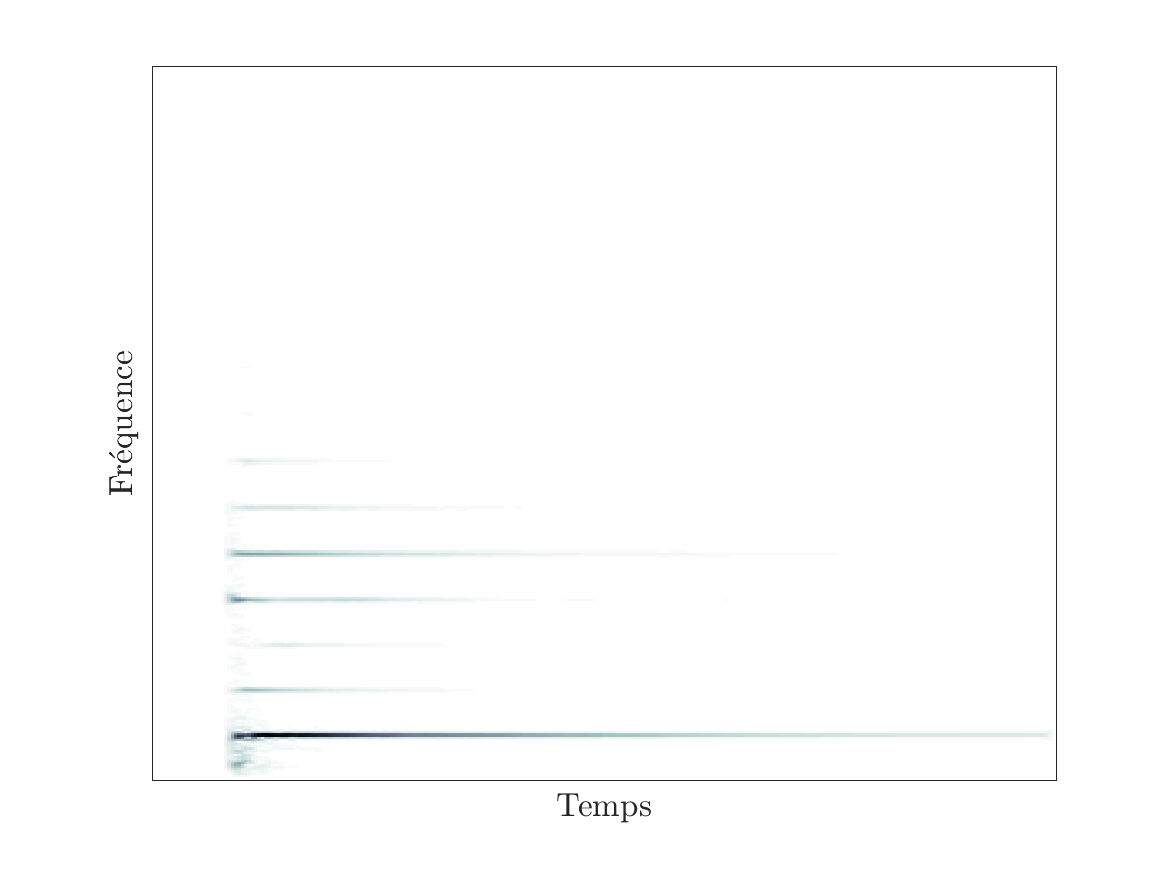
\includegraphics[width=\textwidth]{pianoSpec}
  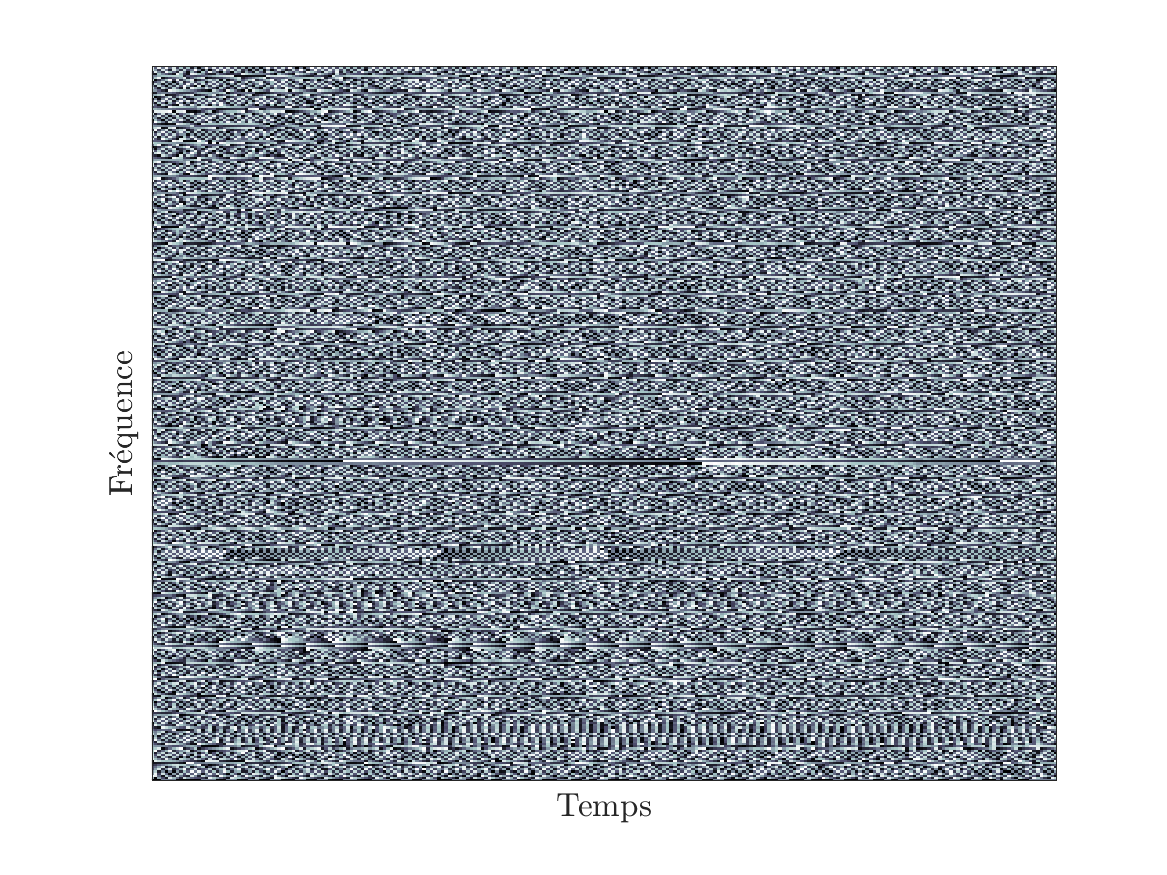
\includegraphics[width=\textwidth]{pianoPhase}
  \caption{Spectrogramme d'amplitude, et de phase d'une note de piano.}
  \label{fig:phase}
\end{marginfigure}

En considérant qu'une partie des sons que l'on cherche à modéliser ont une structure temporelle forte, on s'intéresse à l'estimation des paramètres de composantes périodiques simples, les sinusoïdes. Considérons pour cela un premier signal \og éprouvette \fg constitué d'une sinusoïde de fréquence et d'amplitude constante:
\begin{equation}
  s_s[n] = a_s sin(2\pi f_s/f_e + \phi_s)
  \label{eq:sin_toy}
\end{equation}
Les paramètres d'amplitude et de fréquence de cette composante s'estiment aisément grâce au spectre de Fourier de ce signal :
\begin{eqnarray}
  \hat{f_s} &=&  \frac{M}{N} . f_e\\
  \hat{a_s} &=& S_s[M].3333
\end{eqnarray}
avec
\begin{equation}
  M = \argmax_m | S_s[m] |.
  \label{eq:sin_toy_select}
\end{equation}

Dans le cas de plusieurs sinusoïdes, on remplacera l'équation \ref{eq:sin_toy_select} par une sélection de maxima locaux dans le spectre de puissance et on considèrera l'usage d'une fenêtre de type co-sinusoïdale (hamming, hann, ...) pour améliorer la localité fréquentielle de la transformée\cite{harris1978use}. En effet, considérer le signal sur un intervalle de temps fixé par la largeur de la trame revient implicitement à fenêtrer le signal par une fenêtre rectangulaire qui a des propriétés spectrales non désirables dans le cas multi composantes. Avec des fenêtres co-sinusoïdales, le lobe principal s'élargit, d'où une perte locale de résolution, mais permet de réduire considérablement l'importance des lobes secondaires, ce qui s'avère indispensable dans un contexte multi composantes.
\marginnote{
   \begin{center}
   (a) \\
   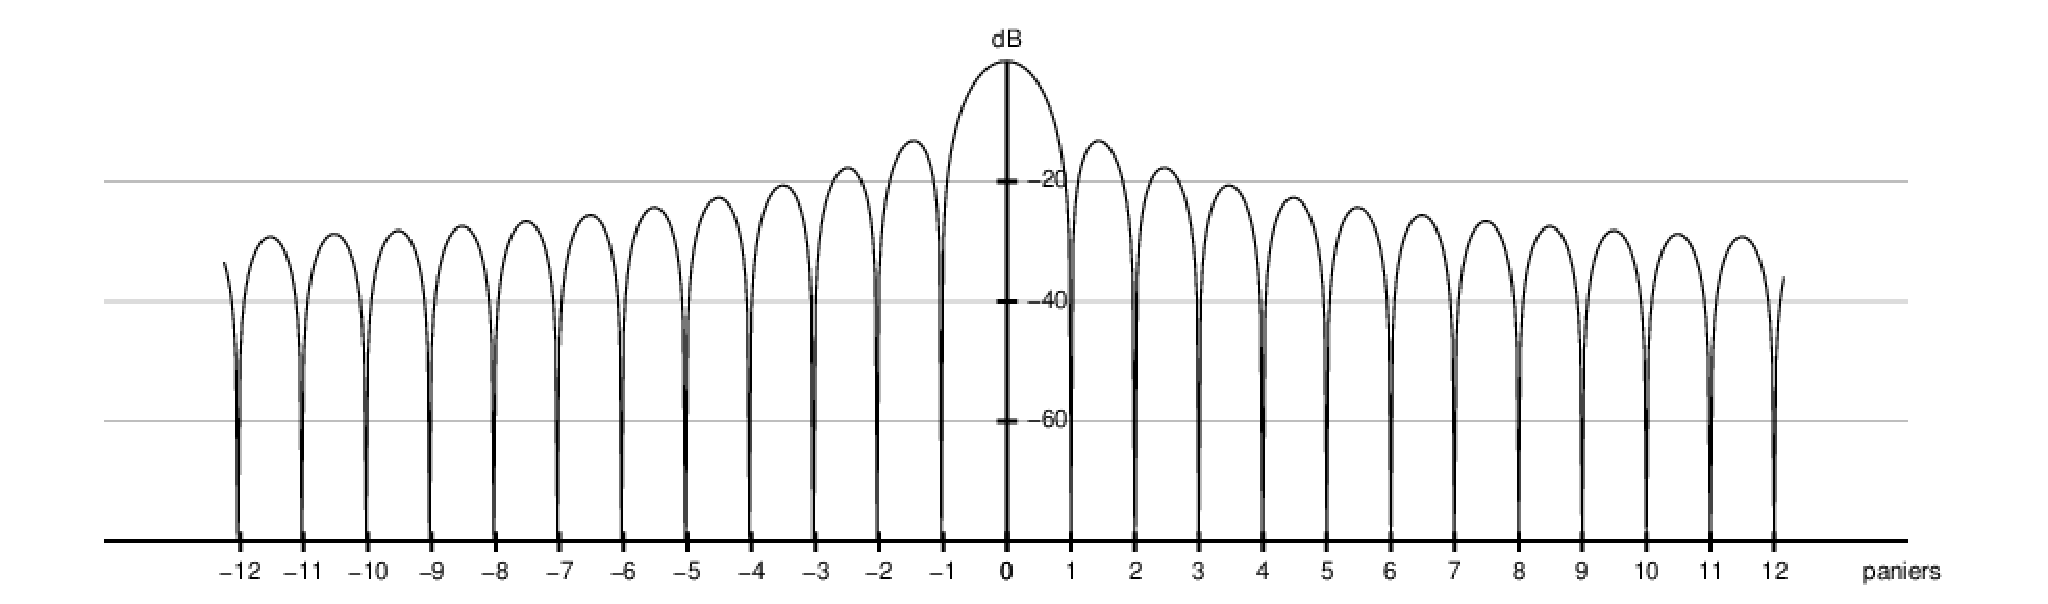
\includegraphics[width=.5\textwidth]{s-rectangularFr} \\
   (b) \\
  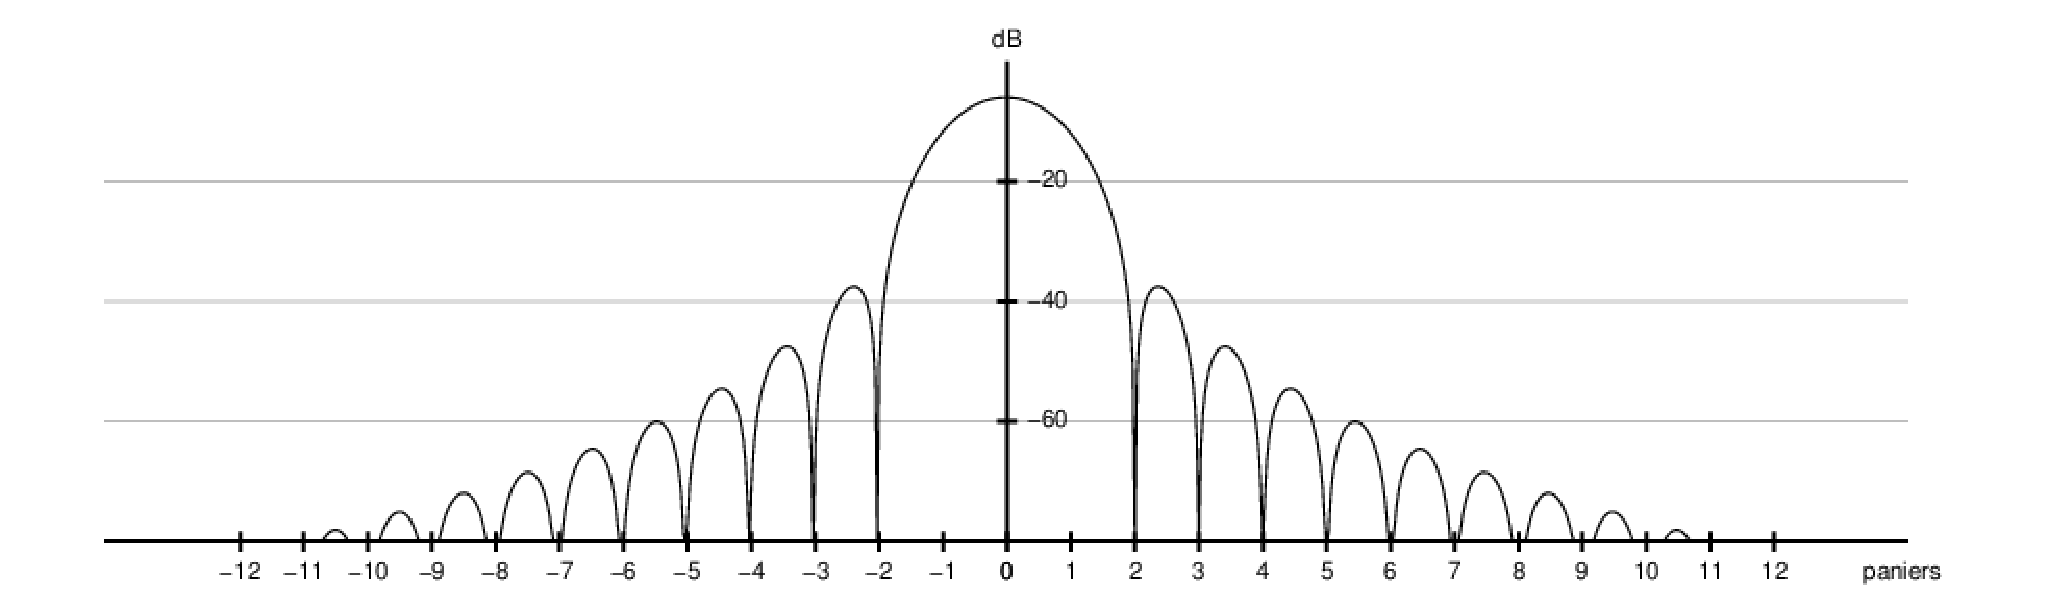
\includegraphics[width=.5\textwidth]{s-hannFr}
 \end{center}
Spectre d'amplitude de la fenêtre rectangulaire (a), et de la fenêtre de Hann (b).
}

On peut améliorer la précision de ces estimations en réduisant le pas de quantification de l'axe fréquentiel. On utilise pour cela la technique du "zero padding", qui consiste à concaténer une série de valeurs nulles au signal observé avant d'opérer la transformation. La transformée s'opérant alors sur plus de points, sa précision en est augmentée.

Un large échantillon de méthodes sont disponibles pour améliorer la précision de ces estimations par d'autres moyens moins directs, comme  celles basées sur le réassignement~\cite{auger1995improving} qui étudient les relations entre le spectre du signal fenêtré et le spectre du signal fenêtré par la dérivée de la fenêtre, ou encore les méthodes basées phase qui étudient les relations entre le spectre du signal et celui de sa dérivée, dont nous avons pu montrer l'équivalence théorique et numérique~\cite{lagrangeJaes07}.

Il est important de bien garder en mémoire que seule la précision est augmentée, la résolution restant dépendante de la largeur du support temporel.  Augmenter l'intervalle d'observation va donc non seulement influer sur la précision, mais également sur la résolution de la transformée. Ainsi, deux sinusoïdes de fréquences proches ne pourront être \og résolues \fg, c'est-à-dire que leurs paramètres pourront être estimés en observant directement le spectre d'amplitude uniquement par l'extension suffisante du support temporel de la transformée.

Considérons un autre signal \og éprouvette \fg constitué cette fois ci d'un dirac :
\begin{equation}
  s_d[n] = \begin{cases}
    a_d \text{ si } n=n_d \\
    0 \text{ sinon}
\end{cases}
\end{equation}
L'estimation du paramètre d'amplitude $a_d$ et de sa position temporelle $n_d$ est triviale dans le domaine temporel :
\begin{eqnarray}
  \hat{n_d} &=&  \argmax_n | s_d[n] | \\
  \hat{a_s} &=&  s_d[\hat{n_d}].
\end{eqnarray}

Cette dernière est par contre beaucoup plus difficile à estimer dans le domaine spectral, du fait du caractère non stationnaire du signal analysé.

Pour palier au caractère non stationnaire à long terme de la plupart des signaux naturels, il est courant d'utiliser la transformée de Fourier à court terme (TFCT). Son principe est d'effectuer une série de transformée de Fourier, chacune sur des fenêtres espacées dans le temps:
\begin{equation}
X[m, t] = \sum_{n = - \infty}^{\infty} x[n] w[n-t] e^{\frac{-2 j  \pi m n}{N}}
\end{equation}
où $w$ est la fenêtre d'observation.

\marginnote{
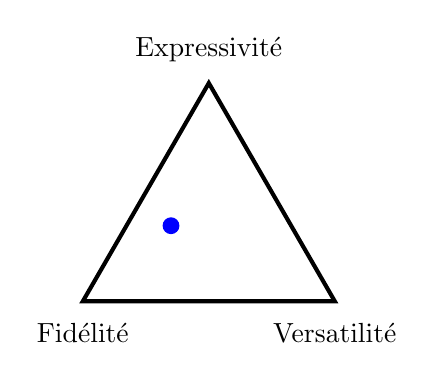
\begin{tikzpicture}[scale=0.8, label distance=1.5mm]
  \coordinate[label=below:Fidélité]  (A) at (0,0);
  \coordinate[label=below:Versatilité] (B) at (4,0);
  \coordinate[label=above:Expressivité] (C) at (2,3.464);
  \draw [line width=1.5pt] (A) -- (B) -- (C) -- cycle;
  \draw [blue, fill=blue, line width=1.5pt] (1.4,1.2) circle [radius=.1 cm];
  \end{tikzpicture}
  Le spectrogramme est à ce jour le compromis le plus apprécié.
}

En prenant le spectre de magnitude de la TFCT, on obtient le bien connu spectrogramme, un outil de manipulation et de visualisation qui trouve son utilité dans de nombreux domaines d'application. L'espoir ici est que les erreurs de modélisation des non stationarités du signal seront négligeables du fait du faible support temporel des fenêtres sur lesquels on applique successivement la TFD. Dans le cas où les fenêtres se recouvrent de moitié, on peut utiliser la transformée en cosinus discret modifiée (TCDM) pour conserver un échantillonnage critique\cite{princen1986analysis}.

En considérant la TFCT, il est alors possible de construire un estimateur \og spectral \fg de la position temporelle de notre dirac :
\begin{equation}
\hat{n_d} = \argmax_t \sum_m X(m, t)
\end{equation}
\'A condition d'utiliser une fenêtre \fg à rampe \og, on peut améliorer la précision temporelle de cet estimateur en réduisant le recouvrement entre fenêtres. La encore, il s'agit d'une amélioration de la précision et non de la résolution. Seule la réduction de l'intervalle d'observation permettra de résoudre la position temporelle de deux diracs proches.

Au travers de ces deux exemples, on voit qu'il est possible d'améliorer dans une certaine mesure la précision des estimations de certaines quantités d'intérêt que l'on peut faire à partir d'un plan temps/fréquence obtenu grâce à la TFCT, mais que les résolutions temporelles et fréquentielles reste conflictuellement contraintes par la taille de la fenêtre choisie. On parle de variables complémentaires pour le temps et la fréquence, au même titre que la position et la quantité de mouvement en mécanique.

Le problème se corse alors sensiblement lorsque l'on considère des signaux qui possèdent une localité temporelle et fréquentielle, ce qui est le cas de la plupart des signaux sonores naturels\marginnote{Un exemple iconique étant la note de piano dont la qualité s'exprime autant du côté de la localité temporelle (netteté de l'attaque) que de la localité fréquentielle (pureté des harmoniques).}.

Il paraît alors naturel de considérer des approches à résolution multiples. Tout le problème consiste alors à trouver une représentation qui maximise le potentiel apporté par la multi résolution en terme de fidélité tout en minimisant la perte en expressivité. En effet, la manipulation de données non régulièrement échantillonnées ou recopiées sous diverses formats, sont un frein à l'aisance de manipulation.

Pour parvenir à une représentation à résolution multiple, l'approche la plus simple conceptuellement consiste à \og effectuer \fg plusieurs DFT de largeur de fenêtre différentes, et ce à intervalle régulier. Cette technique peut se révéler utile dans le cas d'inspection de données ou de prises de décision. Il est par exemple courant, de procéder à des fusions ensemblistes de classifieurs d'architectures équivalentes effectuant leurs prédiction à partir de représentations spectrales de résolution différentes. Dans le cas d'un modèle de son, cela induit malheureusement une perte inacceptable en manipulabilité du fait de la perte d'unicité de la représentation.

Pour éviter cette perte, il est nécessaire de baser notre modèle sur une représentation qui soit à même de partager judicieusement le plan temps / fréquence de manière à mitiger au mieux la contrainte posée par le principe d'incertitude. Un immense travail de la communauté de traitement du signal a été de concevoir ce type de transformée, connue maintenant sous le nom de transformée en \og ondelettes \fg.\cite{mallat1989theory}.

Même si les travaux théoriques dans ce domaine ont permis d'ouvrir considérablement les possibilités en terme de conception, je me  tiendrai ici à la forme la plus courante en traitement du signal qui consiste en une construction d'un banc de filtre dyadique à facteur de qualité constant. Ce banc de filtre est constitué d'un ensemble filtres passe bande à l'octave, \textit{i.e.} la fréquence de coupure supérieure est égale à deux fois la fréquence de coupure inférieure. On obtient alors un pavage alternatif du plan temps / fréquence. Du fait du principe d'incertitude, les paniers ont la même aire, mais le rapport entre résolution fréquentielle et temporelle est optimalement adapté.

\marginnote{
  % \begin{center}
  %   (a) \\
  %
  %   (b) \\
  %
  % \end{center}
Pavage du plan temps/fréquence pour le spectrogramme (a) et la transdformée en ondelettes (b).
}


En considérant que le banc de filtre est construit de manière itérative en partant des hautes fréquences, et en notant que le signal observé est d'une durée limitée, une partie du spectre en basse fréquence ne peut être capturé. On ajoute alors un filtre passe bas dit \og de terminaison \fg qui permet de préserver l'unicité de la représentation. Ce dernier filtre est souvent appelé \og fonction d'échelle \fg. Les sorties de ce banc de filtres peuvent être ensuite re-échantillonnées à une fréquence de Nyquist correspondante à la largeur de la bande d'octave du filtre considéré% QUID DU FILTRE DE TERMINAISON ?
. Comme le montre les travaux pionniers en ce domaine\cite{kronland1987analysis}, l'application de la transformée en ondelettes paraît avoir d'excellentes propriétés pour le traitement de l'audio, en particulier cette capacité à proposer une analyse multirésolution en préservant la propriété d'unicité.

\marginnote{
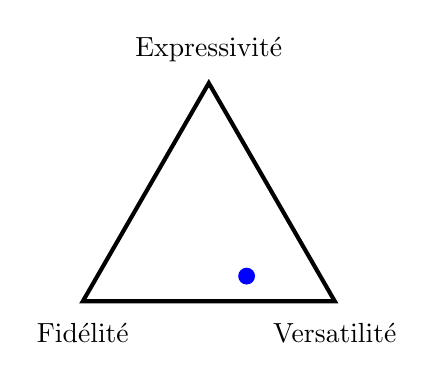
\begin{tikzpicture}[scale=0.8, label distance=1.5mm]
  \coordinate[label=below:Fidélité]  (A) at (0,0);
  \coordinate[label=below:Versatilité] (B) at (4,0);
  \coordinate[label=above:Expressivité] (C) at (2,3.464);
  \draw [line width=1.5pt] (A) -- (B) -- (C) -- cycle;
  \draw [blue, fill=blue, line width=1.5pt] (2.6,.4) circle [radius=.1 cm];
  \end{tikzpicture}
  Les modèles de sons basées sur la transformée en ondelettes sont en théorie plus versatile grâce à la multirésolution, mais peu de travaux démontrent leur expressivité.
}

Quelques décennies plus tard, on peut faire le constat que l'utilisation de la transformée en ondelettes reste marginale en traitement de l'audio. Dépasser ce constat pour amener des éléments concrets nécessiterait une étude approfondie qui sort du cadre de cet exposé. On peut néanmoins avancer quelques éléments de réflexion. Une première explication peut être que les fonctions de bases de la transformée en ondelettes, \textit{i.e.} les réponses impulsionnelles des filtres passe bande ont des formes particulièrement irrégulières, non adaptées à l'audio. On peut en effet aisément retenir cet argument pour des ondelettes de Daubechies de faible longueur, mais devient moins recevable pour des longueurs plus élevées, ou pour les ondelettes de morlet. Cet argument pourrait néanmoins expliquer pourquoi cette transformée à plutôt pris son essor dans le domaine du traitement d'image, où les discontinuités sont beaucoup plus fortes que pour les signaux sonores. En effet chaque contour d'un objet amène une discontinuité importante dans l'espace couleur, qui, dans le cas de la reconnaissance apporte des éléments d'interprétation très importants, et, dans le cas du codage, se doit d'être représenté en détail, sous peine d'engendrer des artéfacts de type \og lissage \fg très pénalisant.

Une seconde explication, finalement peut être plus déterminante, peut avoir trait à la manipulabilité de la transformée. L'interprétation  du spectrogramme est intuitive et permet une manipulation fine du contenu spectral d'un signal audio par des opérations de masquages par exemple, voir la section dédiée à l'\nameref{sec:asa}. L'échantillonnage non régulier en temps et en fréquence de la transformée en ondelettes ne simplifie pas l'expression des transformations que l'ont souhaitent généralement opérer (transposition, étirement, ...). La version filtrée pour obtenir un échantillonnage régulier en temps est plus appropriée, mais au prix de la perte de toute notion de multi-résolution.

% \begin{marginfigure}
%   (a) \\
%   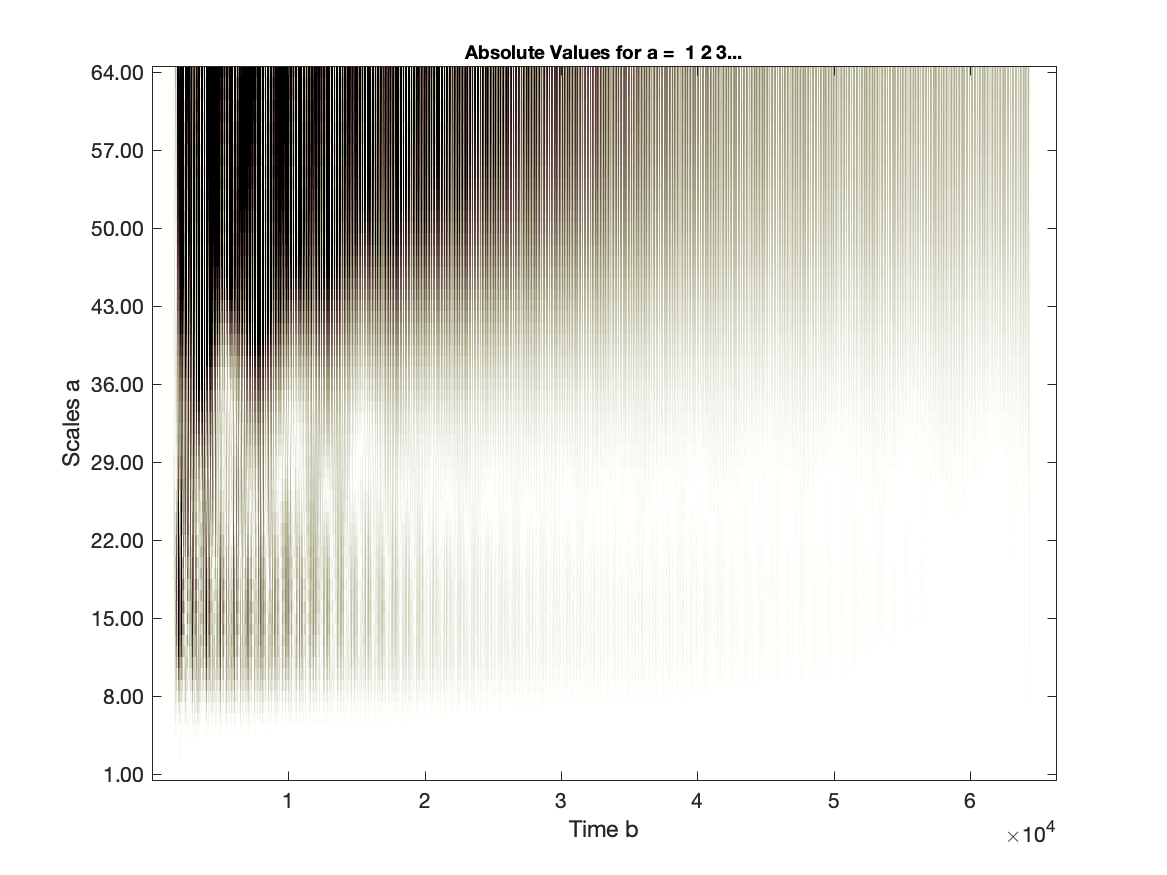
\includegraphics[width=\textwidth]{pianoCwt} \\
%   (b) \\
%   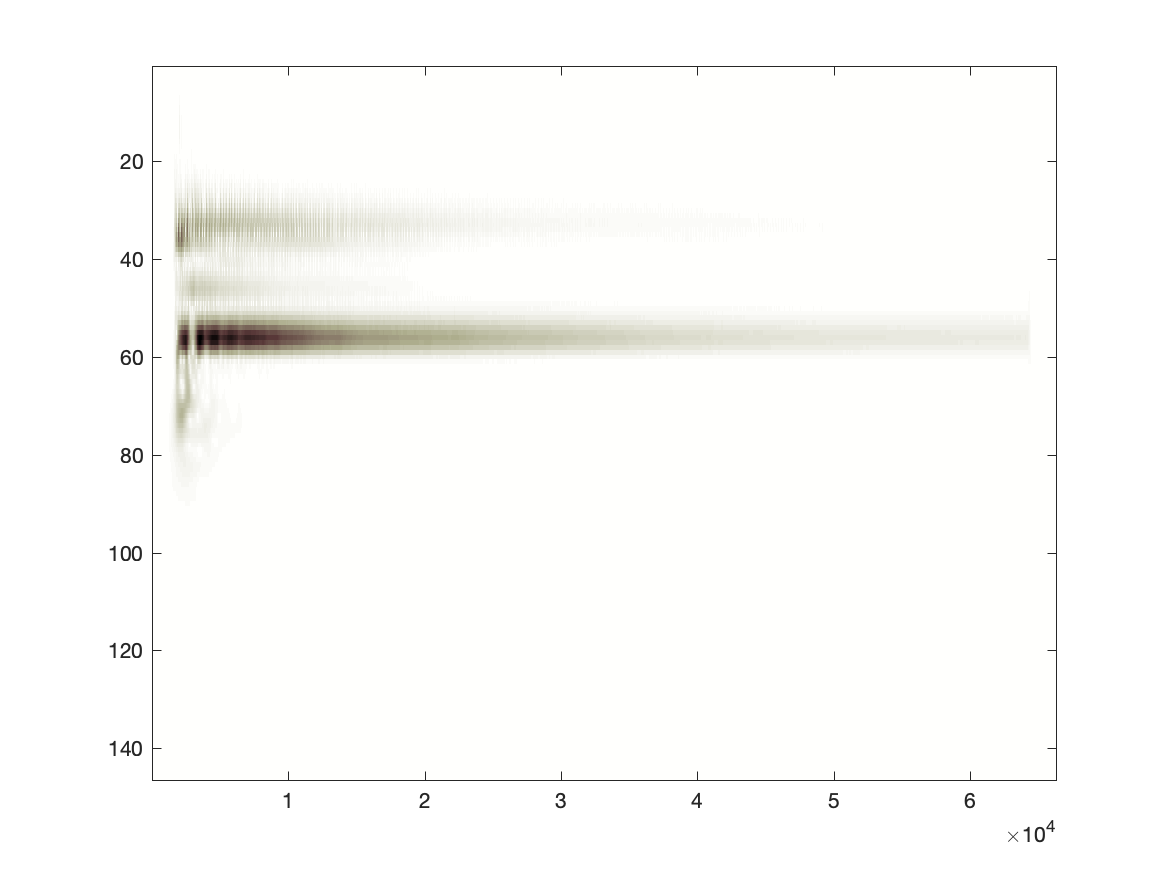
\includegraphics[width=\textwidth]{pianoSca}
%   \caption{transformée en ondelettes (a) et scalogramme (b) d'une note de piano.}
% \end{marginfigure}

En tout état de cause, dans le domaine de l'audio, la grande majorité des systèmes de traitement considère une représentation de type TFCT, avec des paramètres de résolution et de précision constants, adaptés à la tâche. Dans les applications de codage, on trouve des mécanismes à résolution multiple de type alterné, implantés grâce des TCDM à plusieurs largeurs de support\cite{brandenburg1999mp3}. Au sein du codeur, une heuristique détermine parmi les résolutions possibles, la résolution la plus adaptée au vu du signal contenu dans l'intervalle d'observation considéré. Cet échantillonnage non régulier de l'axe temporel permet une meilleure fidélité et flexibilité si l'heuristique est adaptée, ceci au détriment de la manipulabilité, le plan temps/fréquence induit étant non régulier, ce qui n'est généralement pas un facteur limitant dans des chaînes de codage.

On considère donc ici que dans l'intervalle d'observation, une source sonore est dominante et que le type de source est structurée soit de manière temporelle soit de manière fréquentielle. Dans le cas d'un contenu polyphonique avec une structure à la fois en temps et en fréquence, cette approche se révèle bien entendu inopérante. La définition d'une méthode d'analyse/synthèse multirésolution reste donc, avec les éléments présentés ici, un champ de recherche encore largement ouvert.

\section{ \nmu Sinusoïdes à court terme}  \label{sec:sct}

Lorsque l'on observe un spectrogramme un instrument de musique tonal, comme celui d'une note de piano (Figure \ref{fig:phase}), il apparaît clairement que l'énergie est concentrée en un ensemble réduit de zones fréquentielles. On dit que ces signaux sont parcimonieux en fréquence. C'est, dans une certaine mesure le cas de la parole\marginnote{En tout cas, il est clair que la \og charge sémantique \fg est portée par cette partie du signal de la parole, comme le montre les exemples de "sine-wave speech", un nombres réduit de sinusoïdes judicieusement placées aux zones de résonances formantiques suffisent à rendre le signal intelligible \url{http://webpages.mcgill.ca/staff/Group2/abregm1/web/downloadstoc.htm\#23}.}.

En suivant cette observation, on peut modéliser chaque zone de forte énergie du plan temps/fréquence par une composante sinusoïdale à court terme. Pour cela, il est commun d'identifier des maxima locaux dans chaque spectre du spectrogramme pour identifier un ensemble de \og pics spectraux \fg, ou \og atomes \fg temps fréquence. On obtient alors le modèle de son suivant :
\begin{equation}
  S_{ct}(t) = \sum_{c=1}^{C_t} a(c,t) sin(2 \pi f(c,t) t + \phi(c,t))
\end{equation}

Les paramètres de fréquence, d'amplitude, et de phase de chaque atome peuvent être estimées grâce aux techniques évoquées dans la section précédente :
\begin{eqnarray}
\end{eqnarray}


Même si cette technique est motivée par la parcimonie, elle se révèle très robuste à la réduction de cette dernière pour peu que le nombre de composante soit suffisant. En effet, l'expansion de Karhunen Loeve de signaux bruités montre qu'une représentation sinusoïdale de ce type de signaux est valide, à condition que les pics soient suffisamment nombreux et de fréquence suffisamment proche pour que la densité spectrale de puissance dans ces zones varie lentement dans le temps\cite{mcaulay}. Le nombre de composantes par intervalle de temps $C_t$ est donc un facteur déterminant. En pratique, dans un compromis favorisant la fidélité et la versatilité au détriment de l'expressivité, on choisira $C_t$ en fonction de contraintes de complexité, \textit{i.e.} le plus grand nombre possible.

\marginnote{
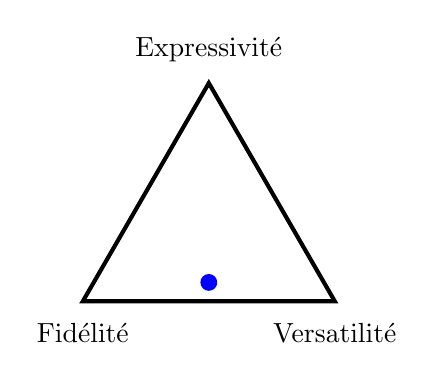
\begin{tikzpicture}[scale=0.8, label distance=1.5mm]
    \coordinate[label=below:Fidélité]  (A) at (0,0);
    \coordinate[label=below:Versatilité] (B) at (4,0);
    \coordinate[label=above:Expressivité] (C) at (2,3.464);
    \draw [line width=1.5pt] (A) -- (B) -- (C) -- cycle;
  \draw [blue, fill=blue, line width=1.5pt] (2,.3) circle [radius=.1 cm];
  \end{tikzpicture}
  La forme d'onde est modèle de son versatile et fidèle mais d'une expressivité limitée.
}




%La précision de ces estimations peut être améliorer par des techniques de sur échantillonage en fréquence et en temps, au détriment du coût de calcul. Ceci étant dit, les limites de cette technique sont bien illustrés dans la figure suivante :

% voice_1024_512.eps

% Ce problème d'estimation dépassant largement la problématique de la modélisation du signal audio, un effort conséquent d'amélioration des ces estimateurs a été effectué par la communauté de traitement du signal. Les approches les plus efficaces et les plus élégantes pour ce faire se basent sur des relations entre les paramètres spectraux de plusieurs transformées de Fourier effectuées après différents traitements du signal observé. La technique du reassignement spectral\cite{auger1995improving} considère le rapport entre la DFT du signal fenêtré et la DFT du signal fenêtré par la dérivée de la fenêtre :
% \begin{equation}
% t
% \end{equation}
% En considérant le rapport de la DFT du signal et celle de la DFT de la dérivée du signal, on obtient une autre série d'estimateurs. On a prouvé l'équivalence théorique de ces dernières à la technique du réassignement, supportée par des expérimentations montrant des performances similaires\cite{lagrangeJaes07}.

Dans un objectif d'expressivité, il est important que  avec l'observation  soit en adéquation avec le modèle utilisé, c'est-à-dire que les composantes sinsuoïdales modélisent des composantes quasi-périodiques présentes dans le signal analysé. En effet, même si une partie bruitée du signal peut être raisonnablement approximée avec des composantes sinusoïdales de fréquence proches et de phase arbitraire, il sera de préserver une bonne qualité d'écoute de signaux modifiés.

Il convient donc dêtre à même de sélectionner parmi les les composantes candidates, celles qui sont les plus appropriées en fonction de critères dits de \og sinusoidalité \fg. Une manière de faire consiste à corréler, pour chaque pic candidat, sa réponse fréquentielle à celle du spectre d'une sinusoïde dont les paramètres sont résultant du processus d'estimation~\cite{peak-selection}. Le degré de corrélation permet alors de quantifier la pertinence du modèle vis-à-vis de l'observation. Une étude comparative semble montrer l'intérêt de cette approche en pratique~\cite{wells2010comparative}. Dans cet algorithme, les références au modèle sont ici construites dynamiquement mais peuvent aussi être échantillonnées. On se rapproche alors du principe des algorithmes de poursuite de sous espaces.

Le principe ici est de s'affranchir des contraintes de la base de Fourier en disposant d'un (très) large dictionnaire d'atomes redondants et de déterminer la combinaison optimale de ces atomes permettant de réduire l'erreur d'approximation. L'algorithme proposé par Zhang et Mallat\cite{mallat1993matching} permet de résoudre efficacement ce problème en considérant un algorithme glouton, où, itérativement, l'atome mis à l'échelle ayant la meilleure corrélation avec le signal résiduel (égal au signal d'origine au début de l'algorithme) est sélectionné.

L'application directe de ce type d'algorithme à des signaux musicaux peut poser des problèmes, dont certains ont été étudiés par Rémi Gribonval. Par exemple, dans le cas de signaux non stationnaire en amplitude, l'algorithme aura tendance à construire des approximations non satisfaisantes.

TODO

La figure illustre deux cas typiques de ce type de non stationarité rencontrés dans les signaux musicaux. Le premier consiste en une composante sinusoidale dont l'amplitude est modulée de manière sinusoidale. C'est une modulation typique d'un tremolo. Le second consiste en une composante sinusoidale dont l'amplitude est modulée exponentiellement. C'est une modulation typique d'une corde frappée ou pincée comme le piano ou le clavecin.

Dans le cas a), l'algorithme MP identifie d'abord une composante avec un support temporel couvrant l'intégralité du signal. Deux autres composantes viennent ensuite annuler certaines parties de cette première. Dans le cas b), le changement abrupt d'énergie étant dificcilement modélisable aves les fonctions de base à disposition, de nombreuses composantes d'annulation sont nécessaires, amenant à un effet de pré écho, l'énergie ajoutée n'étant que partiellement enlevée.

gribonval.png

Pour palier à ces problèmes, des contraintes de non negativité ont été proposé pour améliorer l'algorithme de poursuite\cite{gribonval1996sound}. En réduisant les contributions destructives (enlever de l'énergie amené par des atomes selectionés mais non présente dans le signal d'origine), cette approche est plus efficace au sens où l'énergie globale des atomes (somme des envelopes des atomes) est plus faible cas a)  et plus fidèle cas b).

Il est difficile de critiquer ces approches de poursuites dans le sens où sa pertinence vis à vis de la tâche va grandement dépendre du degré de pertinence du dictionnaire choisi. On notera tout de même que ces approches sont construites avec un objectif d'appromixation et non d'identification. Par exemple dans le cas (a), les deux algorithmes de poursuites sont tout deux à même de bien approximer le signal, mais \og n'identifie \fg pas le phénomène, le dictionnaire n'ayant pas ce type de forme \marginnote{On préfèrera en tout état de cause la seconde approximation pour des raisons de simplicité. PARLER DE L'INDETERMINATION ?}.

A ce titre, on se trouve donc avec un compromis de modèle favorisant la fidélité et la flexibilité, au détriment de la manipulabilité. Il est en effet difficile, dans le cas d'un dictionnaire très largement redondant de déterminer des fonctions simples de manipulation.

Ces approches, comme la transformée en ondelettes, ont trouvés application plutôt dans le domaine du traitement de l'image, où le caractère hautement non stationnaire des transitions entre objets sont très mal approximé par des fonctions régulières comme celle de Fourier.

\section{ \nmu Sinusoïdes à long terme}  \label{sec:slt}

\cite{mcaulay}

L'approche court terme effectue des observations discrètes d'un processus de production sonore qui lui est par essence continu. Dans le cas de nombreux instruments de musique, il est raisonnable de considérer que ce processus continu est approximable par une somme de sinusoïdes dont les paramètres varient \textsl{lentement}\footnote{Typiquement, de l'ordre de la dizaine de Hertz.} dans le temps :
\begin{equation}
t
\end{equation}

En supposant les paramètres connus, le processus de synthèse est aisée à mettre en oeuvre avec les moyens computationels actuels\marginnote{Dans le cas d'un nombre de sinusoide très grand des algorithmes de "pruning" peuvent être mis en place\cite{lagrangeDafx01}.}. Il est également aisé de mette en place des modifications du signal d'intérêt comme la translation, la transposition, ou encore l'étirement, simplement en manipulant les paramètres\marginnote{Ces transformations sont également à faible coût, les paramètres étant échantillonnés à une fréquence environ 1000 fois plus faible que le signal}. On est donc typiquement dans un compromis qui favorise la fidélité et la manipulabilité. Ceci se fait, on le verra par la suite, au détriment de la flexibilité, ce modèle étant applicable à un champ restreint de signaux sonores.

Dans notre étude des algorithmes d'estimation des paramètres long terme, on supposera que le signal analysé est composé d'une ou plusieurs sources dont une grande partie de leur énergie peut être correctement approximée par ce modèle. On fera état ici des approches dites de \og restoration \fg de continuité, qui considèrent connu un modèle court terme du signal analysé mais dont la fiabilité n'est pas pré supposée\marginnote{Ce n'est bien entendu pas la seule approche possible. On peut notamment citer les travaux de Corentin Dubois qui a étudié l'application des techniques de filtrage particulaire pour l'estimation conjointe des paramètres court terme et long terme\cite{dubois2005tracking}, travail étendu à des modèles de sources harmoniques\cite{dubois2007joint}}.


Dans l'article séminal de George Mac Aulay \& al, il est donc proposé \og d'identifier \fg ces composantes long terme en reliant entre eux des atomes de trames successives. L'algorithme proposé est itératif. Supposant un ensemble de composantes long terme à la trame $t$, on va chercher à prolonger ces composantes à la trame $t+1$ en commençant par la composante de plus basse fréquence, tel que la différence entre $$ et $$ est minimale :
\begin{equation}
t
\label{eq:cst}
\end{equation}
Dans un principe d'allocation exclusif, cet atome est dès lors réservé, indisponible pour la suite du déroulement de l'algorithme. Chaque atome non réservé devient alors une composante long terme qui sera potentiellement prolongée aves des atomes de la trame suivante\marginnote{On note ici que la structure de données se complexifie sensiblement par rapport à la plupart de celles introduites avec des outils de traitement du signal canoniques, amenant une approche plus \og informatique \fg à une problématique de traitement du signal. Cette modélisation plus \og riche \fg a permis une flexibilité de manipulation qui a donner lieu à un large ensemble d'heuristiques qui ne seront pas étudiées ici, même si elles ont leur intérêt pour la qualité du rendu sonore de ce type d'approche.}.

La contrainte exprimée par l'équation \ref{eq:cst} favorise des trajectoires fréquentielle constantes. Dans le cas d'un modèle court terme de bonne qualité, par exemple dans le cas d'un signal monophonique à structure harmonique cette heuristique peut être raisonnable. Dans le cas de signaux bruités et/ou polyphoniques, il est utile d'améliorer la finnesse du prédicteur en considérant par exemple un prédicteur linéaire appliqué aux séries temporelles des paramètres long terme. Le faible échantillonage de ces séries temporelles nécessite des estimateurs adaptés comme celui de Burg\cite{burg1968new}.

La contrainte d'évolution lente des paramètres dans le cas d'un modèle stationnaire (prédicteur constant) se traduit nautrellement par un seuil sur le delta de fréquence. L'amélioration du prédicteur nous a également amené à reconsidérer cette étape de sélection.

Les bons résultats en terme de rendu sonore obtenu dans le cas  de la modélisation long terme sous contrainte de débit\cite{lagrangeTaslp06} et l'interpolation de données manquantes\cite{lagrangeJaes05}, montre l'intérêt de la modélisation des modulations long terme, au moins du point de vue perceptif.

Fort de cette observation, Martin Raspaud à étudier un modèle long terme hiérarchique qui permet des manipulations riche comme par exemple de l'étirement temporel de notes vibrées. Le principe est de considérer les paramètres long terme comme des signaux, eux mêmes modélisables comme des sinusoïdes dont les paramètres évoluent (très) lentement en fonction du temps.

D'une grande élégance formelle, d'une grande expressivité et manipulabilité, le modèle long terme n'a pas pu trouver un large spectre spectre d'application du fait d'un défaut clair de versatilité\footnote{On peut citer pour exemple le codeur STS de Phillips qui n'a pas réussi a concurrencer les approches MDCT.}.

\marginnote{
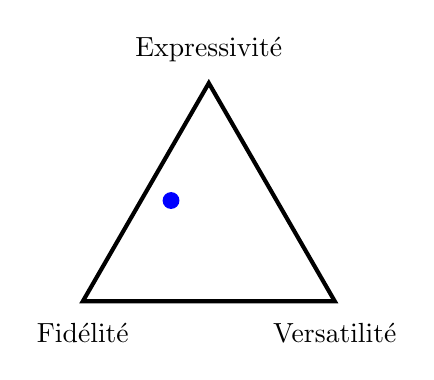
\begin{tikzpicture}[scale=0.8, label distance=1.5mm]
  \coordinate[label=below:Fidélité]  (A) at (0,0);
  \coordinate[label=below:Versatilité] (B) at (4,0);
  \coordinate[label=above:Expressivité] (C) at (2,3.464);
  \draw [line width=1.5pt] (A) -- (B) -- (C) -- cycle;
  \draw [blue, fill=blue, line width=1.5pt] (1.4,1.6) circle [radius=.1 cm];
  \end{tikzpicture}
  Le spectrogramme est à ce jour le compromis le plus apprécié, même si sa versatilité reste limitée.
}

Certaines approches, dites hybrides, consistant à combiner un modèle long terme avec un modèle de bruit et modèle de transitoires ont été proposées pour palier à ce défaut. On tombe alors dans un problème de sélection de modèles que l'on peut espérer mitiger dans le cas d'un signal monophonique\marginnote{on est alors souvent dans le cas d'une analyse experte ou l'intervention humaine est décisive, ce qui peut avoir son intérêt dans certaines applications} mais qui devient  rapidement insoluble dans le cas polyphonique.

EXPLICITER PLUS LES RAISONS ?

\section{ \nmu Temps / fréquence / modulations}  \label{sec:tfm}

S'il est clair que la décomposition fréquentielle est de première importance, la manière dont l'énergie module au court du temps au sein de ces bandes de fréquences l'est également \marginnote{On peut citer pour exemple le son éminement désagréable d'un moteur thermique deux temps (type mobylette) qui part le mouvement mécanique induit une modulation typique.}. L'importance perceptive de ce type de modulations est particulièrement bien exemplifiée par un exemple sonore produit par John Chowning où des sinusoides d'amplitude et fréquence au début constantes sont ensuite modulées par un signal synthétique composé d'une composante sinusoidale (pour le vibrato) et d'une composante stochastique. Ce signal modulant est ensuite mis à l'échelle pour chaque harmonique. Il est important de considérer que même si ce signal modulant a été judicieusement choisi, il n'est pas issu d'un processus d'estimation à partir de signaux réels.

L'écoute montre clairement que le caractère naturel, voisé, est sensiblement plus élevé avec l'ajout de la modulation \footnote{Ce stimuli est disponible ici \url{http://webpages.mcgill.ca/staff/Group2/abregm1/web/snd/Track24.mp3} pour écoute sur le site de Al Bregman dédié à l'ASA. Les spécificités techniques du porcessus de synthèse sont décrites ici : \url{http://webpages.mcgill.ca/staff/Group2/abregm1/web/downloadstoc.htm\#24}.}.

\subsection{Modèles perceptifs}

Complétons nos connaissances en prenant cette fois ci, non plus un point de vue physique mais physiologique. L'étude des éléments physiologiques en charge du traitement de ces modulations est relativement récente car probablement sensiblement plus difficile a investiguer. On a néanmoins une bonne confiance dans le fait que le système auditif des mammifères dispose d'éléments de traitement dédiés à cette tâche. On peut notamment citer le modèle de Torsten Dau\cite{dau1997modeling} et celui de Shihab Shamma\cite{fritz2003rapid} qui étend le modèle de Dau en ajoutant une troisième dimension : l'échelle.

Shihab Shamma a étudié certaines neurones du cortex auditif primaire du furet, plus particulièrement ce que l'on appelle leur champs de réponse spectro/temporellle ou "spectro-temporal receptive fields" (strf). L'animal est contraint au niveau du crâne, et par opération chirugicale, une aiguille permettant de mesurer l'activité électrique est insérée dans le crâne de l'animal et judicieusement placée. Par exposition d'un ensemble de stimuli comportant des modulations, il est alors possible de mesurer ces strf. Au vu de ce type de réponses, Un modèle de traitement de signal est ensuite proposé.

Dans ce modèle, le signal est donc tout d'abord décomposé sur l'axe fréquentiel. La sortie étant un équivalent du spectrogramme qui est ensuite décomposé une nouvelle fois fréquentiellement en temps et en fréquence grâce à des ondellettes bi-dimensionnelles paramétrées avec un facteur d'échelle. La dimension de l'échelle permet de définir le nombre de bandes qui sont conjointement utilisées pour effectuer cette seconde analyse fréquentielle \marginnote{Ces modèles sont bien entendu sujet à débat dans la communauté de neurophysiologie. Par exemple, le facteur d'échelle est pour Dau non nécessaire pour expliquer les données recueillies grâce à son protocole expérimental.}.

\subsection{\nmu Scattering d'ondelettes}  \label{sec:scattering}

En prenant un point de vue mathématique cette fois ci, Stéphane Mallat a proposé un modèle conceptuellement proche du modèle computationel des STRF proposé par Shihab Shamma. En mathématiques appliquées, et plus particulièrement dans le domaine des sciences des données, on cherche à construire des représentations qui aient de bonnes propriétés d'invariance et de stabilité aux déformations. C'est à dire que l'on souhaite que pour une représentation $\phi(x)$ d'un signal $x$ et d'un signal déformé $\tilde x$ :
\begin{itemize}
  \item invariance : $\phi(\tilde x) = \phi(x)$
  \item stabilité : $ \vert \phi(\tilde x) - \phi(x) | < \epsilon $
\end{itemize}

Précisons ces notions en prenant quelques exemples. Lorsque l'on cherche à reconnaitre l'instrument de musique qui a joué la note enregistrée, on souhaite généralement disposer d'une représentation du signal de cette performance qui soit invariante à certains aspects de la performance comme :
\begin{enumerate}
  \item un changement d'amplitude
  \item une translation en temps
  \item un étirement en temps
\end{enumerate}
En effet, pour la tâche pré-citée, que la note ait été jouée plus ou moins proche du microphone\footnote{J'écarte ici pour la simplicité du discours les aspects de nuances qui ont une influence non négligeable sur le timbre.}, à un instant donné ou quelques secondes plus tard, à une hauteur donnée ou une autre, pour une durée plus ou moins longue ne devrait pas (trop) modifier notre représentation.

L'invariance au volume est obtenue de manière triviale en normalisant les signaux que l'on souhaite comparer. L'invariance à la translation en temps se traduit dans le domaine de Fourier en une invariance à la translation de phase par la prise du module. On souhaite généralement que l'invariance au volume et à la translation soit complète. En ce qui concerne l'invariance à l'étirement temporel, on souhaite généralement plus que la représentation soit stable à la déformation.

Il est clairement explicité dans\cite{anden2014deep} pourquoi le spectre de magnitude de Fourier n'est pas stable à même un petit étirement temporel. En effet, l'impact de l'étirement selon l'axe des fréquences n'est pas le même. Si un petit étirement déplacera d'une petite quantité les fréquences basses, les fréquences le seront beaucoup plus. Prenons le cas classique d'un signal harmonique de fréquence de fondamentale $440 Hz$, un étirement temporel va réduire la valeur de cette fréquence à disons $430 Hz$ pour un delta de $10 Hz$. Ce delta sera $n$ fois plus grand pour la $nième$ harmonique soit $100 Hz$ pour la dixième harmonique. Pour une transformée de Fourier avec des paniers d'une dizaine de Hertz, la différence entre les deux spectres va croitre très rapidement avec delta car l'énergie des harmoniques supérieures va très vite sortir des paniers où l'énergie des harmoniques se plaçait initialement.

Pour être plus stable à ce type de déformation, il convient alors de \og délocaliser \fg les hautes fréquences de manière plus conséquente que les basses. Suivant les communautés, on obtient cette délocalisation progressive sur l'axe des fréquences avec des transformées à Q constant, de type tiers d'octave (acoustique), des Mels ou des Barks (parole)\marginnote{Cette étude est à mon sens d'importance, car elle permet de placer un cadre mathématique pour mieux expliquer ce qui a été empiriquement vérifié dans de nombreux domaines du traitement de l'audio et motivés jusqu'ici par des arguments essentiellement neuro mimétiques.}.

En se plaçant dans le cadre des ondelettes, on obtient ce type de représentation en délocalisant en temps toutes les bandes de fréquence ce qui induit une perte d'information qu'il convient de compenser. Le principe du scattering permet de répondre élégamment à ce problème en cascadant des opérations de décomposition et en utilisant chaque niveau de décomposition pour produire une représentation compacte et informative \marginnote{En dissociant ainsi décomposition et représentation, on peut préserver certaines propriétés d'intérêts comme par exemple l'inversibilité pour la décomposition et la stabilité pour la représentation.}.

Le scattering au premier ordre est donc équivalent en termes conceptuels à une transformée à Q constant. En décomposant les sorties un banc de filtres en ondelettes avec un autre banc de filtres, on capte alors l'information de modulation, \textit{i.e.} comment l'énergie fluctue dans une même bande fréquence. On a vu précédemment l'importance de ce type de modulation pour la perception. Il est donc opportun de d'étudier l'apport du second ordre pour une représentation riche du signal sonore\marginnote{Le processus de cascade. Le troisième ordre est conceptuellement difficile à appréhender et a encore été peu étudié, pour les raisons suivantes 1) pratique : l'énergie au troisième ordre est très faible, 2) neuro-mimétique : aucun modèle perceptif n'explicite un troisième ordre de traitement.}.

L'apport du second ordre a été démontré expérimentalement pour des tâches de modélisation\cite{anden2014deep}.

Nous avons complétés cette investigation en considérant une tâche pertinente pour notre propos : l'étude de la représentation des sons d'instruments de musique du répertoire en considérant des modes de jeux étendus. En effet, si la reconnaissance de l'instrument est considérée comme un problème résoluble par une représentation à Q constant\cite{}, la reconnaissance du mode de jeu\footnote{et par la même d'une notion plus fine de la notion de timbre musical} comporte des éléments de modulations qui ne sont pas aisément capturés par une représentation à Q constant ou un scattering d'ondelettes à l'ordre un. On montre en effet que l'ajout de l'ordre 2 permet une bien meilleure identification du mode de jeu et permet de proposer au compositeur à la recherche d'un certain timbre, d'une investigation plus aisée d'une grande base de données de sons instrumentaux\cite{}.

En terme d'architecture de décomposition, le scattering suit une organisation de type réceptive, fréquence d'abord et temps ensuite. On verra dans la partie suivante un modèle prenant une approche de type source / filtre donc temps et fréquence ensuite et qui est à ce titre plus directement tourné vers la synthèse.

\section{ \nmu Synthèse modale}

En se référant plutôt aux processus physiques de production sonore, les approches modales permettent de proposer des méthodes efficaces pour des outils de synthèse dédiés.

Ces modèles se basent sur un modèle de production de type source / filtre, où la source est généralement décrite en terme de propriétés temporelles, et le filtre en terme de propriétés fréquentielles. Pour un signal de parole, on considèrera que la source peut être soit un train d'impulsions résultant de l'ouverture périodique de l'organe phonatoire nommé, à tort,  cordes vocales pour la production des sons voisés (voyelles) soit un signal stochastique résultant de la compression du flux respiratoire pour la production des sons plosives ou sifflants (consonnes).

Le modèle source / filtre décorrelle donc naturellement la contribution de l'excitateur et celle du résonateur, ce qui est particulièrement attrayant lorsque l'on recherche un modèle de son permettant une bonne capacité d'interaction. Pour peu que les modèles utilisés pour les deux parties (source et filtre) soit bien adaptés, on obtient des modèles de sons qui sont souvent fidèles et expressifs\cite{aramaki2006analysis}. La flexibilité reste malheureusement en deca, car le changement de structures pour la source et le filtre ainsi que leurs modes d'interactions nécessitera le plus souvent des adaptations d'ordre computationels si ces changement sont conséquents.

Nous avons par exemple étudié ce type de modèle pour la synthèse de sons de roulements. Ces sons présentent un challenge pour ce type de synthèse car l'interaction entre la bille et la surface sur laquelle elle roule est complexe.

\cite{LagrangeTasslp10}

 validation perceptive

\cite{Murphy11a}

marseille\cite{conan2014synthesis}

On se trouve ici à l'intersection entre modélisation statistique et modélisation physique, dans le sens où l'architecture du modèle de son suit un modèle de production.



On trouve avec ce type de modèle deux propriétés d'importance. En premier lieu, la causalité. Au niveau du modèle de synthèse, un échantillon est strictement considérée comme une composante des échantillons précédents.  En second, cette approche met l'accent sur les propriétés de filtrage des composantes modales, il ne s'agit pas ici de synthétiser un signal riche à partir d'une représentation complète du signal, mais plutôt d'exploiter un modèle source / filtre avec une implantation dédiée de ces deux modules en fonction de la tâche visée.

Même si ce type d'approche est utilisée de manière assez marginale, elle garde à mon sens un intérêt historique pour mettre en perspective les approches modernes décrites dans la suite.


\section{ \nmu Conclusion}

POSER LES PROBLEMATIQUES

NOTER LES AMELIORATIONS






TODO EN DISCTUER UNIQUEMENT EN CONCLUSION

Cette revue des modèles de sons nous a permis d'identifier deux verrous qu'il semble difficile de résoudre de manière conjointe.

Rappelons ici les trois propriétés souhaités :
\begin{enumerate}
  \item
  \item
  \item versatile
\end{enumerate}

En suivant cet ordre, on peut procéder à la constitution d'un \og cahier des charges \fg du modèle idéal qui serait le suivant :
\begin{enumerate}
  \item multirésolution
  \item causal

\end{enumerate}

\cite{wavenet}

techniques introduites initialement pixelrnn \marginnote{La précédence d'application de nouvelle technique entre le domaine de l'image et le domaine de l'audio est quasiment toujouts observée. C'est à mon avis du à deux facteurs, l'utilité et la facilité. Nombreuses sont les applications qui necessitent du traitement de l'image, notamment à cause de la prédominance du visuel dans notre approche du réel. La facilité vient de nombreux facteurs. Un premier est qu'il est plus facile d'approcher les dimensions spatiales qui sont cohérentes entre elles. Le temps est notoirement plus complexe à modéliser. Un second est que l'oeil est notoirement plus tolérant que l'oreille. On peut donner comme exemple sur ce dernier point le morphing. Une simple somme pondérée entre deux images judicieusement cadrée permet d'obtenir des résultats appréciables. Ce type de technique est ineffective en audio où le morphing est encore un problème non résolu.}.

Les résultats obtenus en terme de qualité perceptuelle nous invite à étudier cette approche novatrice qui semble apporter des réponses à la problématique non résolue d'une méthode d'analyse synthèse multi résolution qui soit à la fois fidèle, expressive et versatile.

présentation du principe de traitement de l'information.

  réseaux neuronaux, présentation avec une optique traitement du signal (LIRE PAPIER MALLAT) \marginnote{neuromimétisme structurel pour les unités et les réseaux, question du conditionnnement chimique, et des mécanismes de prédiction et d'apprentissage. Mécanismes totalement distincts dans les modèles computationnels, pas d'équivalent en neuro sciences.}

présentation de l'architecture

vocoder

certains aspects peuvent trouver des fondements dans des modèles de sons existants

causalité stricte

source filtre

conditionnement lent

Certains aspects de l'architecture sont spécifiques.

Le plus important étant que l'écoute montre l'absence d'artefacts typiques d'une chaîne de traitement spectral mono résolution comme la tfct.

question du conditionnement



Ces points, et de nombreux autres comme l'impact des fonctions de non linéarité sur la qualité du signal généré sont des questions passionnantes, largement ouvertes en terme de compréhension scientifique.

De part la qualité du traitement et la versatilité de ces approches, leur étude constitue pour moi une opportunité pour la communauté traitement du signal. C'est d'autant plus important que la communauté d'apprentissage artificiel traverse actuellement une crise de sens. Ainsi, une vision fondée sur les principes du traitement de l'information, l'équilibre entre empirique et formalisme. Tout ces éléments qui constitue les fondements du traitement du signal sont à mon avis de grand intérêt pour répondre à des questions, qui au vu du champ d'application extrêmement vaste de ces outils, dépasse les problématiques de la seule communauté des sciences des données, pour devenir un enjeu de société.


approche source filtre <> latent code
